\documentclass[a4paper,10pt, nofootinbib]{article}
\usepackage[width=15.5cm, left=3cm, top=2.5cm, right=1cm, left=2cm, height= 24.5cm]{geometry}
\usepackage[spanish]{babel}
\usepackage[utf8]{inputenc}
\usepackage[T1]{fontenc}
\usepackage{xspace}
\usepackage{xargs}
\usepackage{fancyhdr}
\usepackage{lastpage}
\usepackage{caratulaMetNum}
\usepackage[bottom]{footmisc}
\usepackage{amssymb}
\usepackage{algorithm}
\usepackage[noend]{algpseudocode}

\usepackage{graphicx}
\usepackage{sidecap}
\usepackage{amsmath}


%%fancyhdr
\pagestyle{fancy}
\thispagestyle{fancy}
\addtolength{\headheight}{1pt}
\lhead{Métodos Numéricos: TP1}
\rhead{$2º$ cuatrimestre de 2015}
\cfoot{\thepage\ / \pageref{LastPage}}
\renewcommand{\footrulewidth}{0.4pt}

%%caratula
\materia{Laboratorio de Métodos Numéricos}
\titulo{Trabajo Práctico Número 1}
\subtitulo{Con 15 $\theta$'s discretizo alto horno}
%\grupo{Grupo 12}
\integrante{Ciruelos Rodríguez, Gonzalo}{063/14}{gonzalo.ciruelos@gmail.com}
\integrante{Costa, Manuel José Joaquín}{035/14}{manuc94@hotmail.com}
\integrante{Gatti, Mathias Nicolás}{477/14}{mathigatti@gmail.com}

\abstracto{Descripcion del Tp}

\palabraClave{Eliminación gaussiana}
\palabraClave{factorización LU}
\palabraClave{discretización}
\palabraClave{key4}

\begin{document}
\maketitle
\section{Introducción teórica}

El objetivo del presente informe es resolver un problema práctico mediante el modelado matemático del mismo. Este problema consiste en considerar la sección horizontal de un horno de acero cilíndrico, y dadas las temperaturas en el interior y en el exterior de este, analizar si se encuentra en peligro o no.

Para ello, se debe encontrar una cierta isoterma, que si se encuentra muy cerca (para algún significado de la palabra muy) de la pared del horno, consideraremos que el sistema se encuentra en peligro.

Para modelar la difusión de la temperatura, utilizaremos la ecuación de Laplace.

\begin{equation}\label{eq:calor}
\frac{\partial^2T(r,\theta)}{\partial r^{2}}+\frac1r \frac{\partial^2 T(r,\theta)}{\partial r} + \frac{1}{r^2} \frac{\partial T(r, \theta)}{\partial \theta^2} = 0.
\end{equation}

Como puede verse en la ecuación \ref{eq:calor}, esta ecuación depende de variables que son continuas, lo que es matemáticamente válido, pero computacionalmente imposible (a menos que se haga simbólicamente) de calcular.

Para resolver este problema computacionalmente, debemos discretizar el dominio del problema en coordenadas polares. Por eso consideramos una particion $0 < \theta_0 < \theta_1 < ... < \theta_n = 2\pi$ en $n$ ángulos discretos, con $\theta_i - \theta_{i-1} = \Delta\theta$ constante, y una partición $r_i = r_0 < r_1 < ... < r_m = r_e$ en $m+1$ radios discretos con $r_j - r_{j-1} = \Delta r$ para $j = 1,...,m$.

Entonces ahora, aproximadoo las derivadas numéricamente utilizando idea del cociente incremental, podemos obtener un sistema de ecuaciones linales que describa el sistema. La formulación detallada de la formulación del sistema se encuentra en el desarrollo.

Para resolver estos sitemas, utilizaremos los dos métodos vistos en clase, eliminación Gaussiana y factorización LU. Además, como explicaremos mejor y también demostramos en el anexo, podemos realizar estos métodos sin utilizar pivoteo, dado que nunca aparecerá ningun $0$ en la diagonal cuando triangulemos la matriz.




\newpage

\section{Desarrollo}
\subsection{Convenciones}
De aquí en adelante, si no se aclara otra cosa, se asumen las siguientes convenciones:
\begin{itemize}
\item$r_i$ es el radio que va del centro del horno al borde interno de la pared, mientras que $r_e$ es el radio considerando el borde externo;
\item$n$ es la cantidad de ángulos discretos ($0=\theta_0 <\hdots< \theta_{n-1} = 2\pi - \Delta \theta$) en los que se particiona la pared;
\item$m+1$ es el total de radios discretos ($~{r_i=r_0<\hdots<r_m=r_e}$); 
\item$t_{k,j} = T(r_k, \theta_j)$, donde $T$ es la función de temperatura de la pared (que desconocemos);
\item$b\in \mathbb{R}^{n\times (m+1)}: b = (b_0, b_1, \hdots, b_{(n\times (m+1))-1})$ será el vector de términos independientes del sistema que plantearemos luego (veremos que la dimensión escogida es correcta). 
\end{itemize}
\subsection{Métodos numéricos usados}
\label{sec:metodos}
A partir de la ecuación del calor de Laplace y las discretizaciones de las derivadas parciales dadas en el enunciado del presente trabajo práctico, se puede obtener un sistema de ecuaciones donde las soluciones son las temperaturas en los puntos de la discretización. 
Es decir que el problema de hallar la isoterma se reduce a dos sub-problemas: el primero es resolver efectivamente el sistema planteado, mientras que el segundo consiste en usar las temperaturas halladas para estimar la posición de la isoterma.\\
Para resolver el sistema haremos uso de los métodos de eliminación gaussiana y la factorización LU, para luego poder contrastar su eficiencia ante distintas situaciones. Adicionalmente, realizaremos una variación de cada método para aprovechar una de las características propias de la matriz del sistema.\\
Para hallar la posición de la isoterma (de temperatura $t_{iso}$), dado un ángulo $\theta_j$ de la discretización, lo que haremos es buscar dos radios, $r_k$ y $r_{k+1}$, tales que $t_{k+1,j} \leq t_{iso} \leq t_{k, j}$. A partir de estos dos valores, facilmente podemos realizar un ajuste lineal considerando la recta de pendiente $m = \dfrac{t_{k,j}-t_{k+1,j}}{\Delta r}$ que pasa por $(r_k,t_{k,j})$ y $(r_{k+1}, t_{k+1,j})$. Para una explicación más detallada ver el apéndice ?????.

  
\subsection{Armado del sistema de ecuaciones y su matriz asociada}
\label{sec:armado-sistema}
Tenemos un sistema con $n\times(m+1)$ incógnitas.

Primero contamos con $n$ variables, los $t_{0,j}$ con $j = 0,1,\hdots, n-1$ (es decir, las temperaturas interiores), cuyos valores conocemos pues nos son dados como inputs. Lo mismo sucede con $t_{m, j}$ para $j = 0,1,..., n-1$ (temperaturas externas).
Luego, para las temperaturas interiores sabemos gracias a la función de Laplace y a la discretización de las derivadas que vale 

$\dfrac{t_{k-1,j} - 2t_{k,j} + t_{k+1,j}}{(\Delta r)^2} 
+ \dfrac{1}{r_k} \times \dfrac{t_{k,j} - t_{k-1,j}}{\Delta r}
+ \dfrac{1}{r_{k}^2} \times \dfrac{t_{k,j-1} -2t_{k,j} + t_{k,j+1}}{(\Delta \theta)^2} = 0$\\

Reescribiendo convenientemente la ecuación de arriba nos queda que 

\begin{equation}
\label{eq:laplace-discreto}
\dfrac{r_k - \Delta r}{r_k (\Delta r)^2} t_{k-1, j} +
\dfrac{1}{r_k^2(\Delta \theta)^2} t_{k, j-1} +
\dfrac{r_k \Delta r (\Delta \theta)^2 - 2(\Delta r)^2}{r_k^2 (\Delta r)^2 (\Delta \theta)^2} t_{k,j} +
\dfrac{1}{r_k^2(\Delta \theta)^2} t_{k, j+1} +
\dfrac{1}{(\Delta r)^2} t_{k+1,j}  = 0
\end{equation}

Hay que distinguir dos casos bordes que deben tratarse un poco diferente: si $j = 0$ entonces en lugar de $t_{k, j-1}$ se usa $t_{k, n-1}$, mientras que si $j = n-1$ en lugar de $t_{k, j+1}$ va $t_{k, 0}$.

Vale destacar que si bien todos los coeficientes dependen de la distancia al centro del horno ($r_k$), ninguno lo hace respecto del ángulo concreto en que se encuentra el punto. Esto resulta muy razonable si tenemos en cuenta que el valor del ángulo depende exclusivamente del sistema de referencia escogido (dónde ubicamos el ángulo 0), mientras que dado un punto de la pared es lógico que su temperatura no dependa del sistema de referencia escogido para su medición.

Para facilitar la lectura, de ahora en adelante llamaremos a los coeficientes de la ecuación (\ref{eq:laplace-discreto}): 
\begin{itemize}
\item $a_k = \dfrac{r_k - \Delta r}{r_k (\Delta r)^2}$ 
\item $b_k = \dfrac{1}{r_k^2(\Delta \theta)^2}$ 
\item $c_k = \dfrac{r_k \Delta r (\Delta \theta)^2 - 2(\Delta r)^2}{r_k^2 (\Delta r)^2 (\Delta \theta)^2}$ 
\item $d_k = \dfrac{1}{(\Delta r)^2}$
\end{itemize}

Pensamos ahora el orden que le daremos a los puntos de la discretización. Este será el orden en el que escribiremos las ecuaciones. Sin demasiadas complicaciones, un orden razonable es primero por ángulo (desde $\theta_0$ y avanzando en sentido antihorario) y luego por radio (de menor a mayor) respetando el orden relativo previo. Luego, dado un $t_{k,j}$ para obtener su posición (contada desde 0) en este orden debemos realizar la siguiente cuenta
\begin{equation}
\label{eq:posicion}
	posicion(t_{k,j}) = k\times n + j
\end{equation}

La cantidad total de variables es $n\times(m+1)$ (cantidad de ángulos por cantidad de radios), y como para cada una podemos o bien plantear la ecuación \ref{eq:laplace-discreto}, o bien ya conocemos su valor, podemos armar un sistema de $n\times(m+1)$ ecuaciones lineales.

A continuación presentamos el sistema de ecuaciones: 

\begin{equation}
\label{eq:sisecu}
  \left\lbrace
  \begin{array}{l}
     t_{0,0} = b_0 \\
     t_{0,1} = b_1 \\
     \vdots\\
     t_{0,n-1} = b_{n-1} \\
		 a_1 t_{0,0} + c_1 t_{1,0} + b_1 t_{1, 1} + b_1 t_{1, n-1} + d_1 t_{2, 0} = 0 = b_{n}\\
		 a_1 t_{0,1} + b_1 t_{1, 0} + c_1 t_{1,1} + b_1 t_{1,2} + d_1 t_{2,1} = 0 = b_{n+1} \\
		 \vdots\\
		 a_1 t_{0,n-2} + b_1 t_{1, n-3} + c_1 t_{1,n-2} + b_1 t_{1,n-1} + d_1 t_{2,n-1} = 0 = b_{2(n-1)} \\
		 a_1 t_{0,n-1} + b_1 t_{1, 0} + b_1 t_{1, n-2} + c_1 t_{1,n-1} + d_1 t_{2, n-1} = 0= b_{2n - 1}\\
		 a_2 t_{1,0} + c_2 t_{2,0} + b_2 t_{2, 1} + b_2 t_{2, n-1}  + d_2 t_{3, 0} = 0 = b_{2n}\\

		 a_{m-1} t_{m-2,n-1} + b_{m-1} t_{m-1,n-1} + c_{m-1} t_{m, n-1} + d_{m-1} t_{m-1, n-2} + d_{m-1} t_{m-1, 0} = 0 = b_{n\times m -1}\\
		 t_{m,0} = b_{n\times m}\\
		 \vdots\\
		 t_{m, n-1} = b_{n\times (m+1)-1}
		 
  \end{array}
  \right.
\end{equation}

$b$ tiene valores pasados por el ususario en las primeras $n$ posiciones y en las $n$ últimas, siendo el resto todos ceros.

Como primera observación importante notemos que el valor de cada $t_{k,j}$ ($1\leq k < m$) depende exclusivamente del valor de sus cuatro vecinos, lo que permite prever que cada fila de la matriz asociada tendrá sólo cinco elementos distintos de 0.

Para realizar la siguiente observación primero veamos un ejemplo concreto. Consideremos la siguiente discretización con $n = 4$ (particionamos la pared en cuatro ángulos iguales) y $m = 3$ (4 radios en total). El sistema tendrá entonces $4\times (3+1) = 16$ variables, con 16 ecuaciones. En este caso, el sistema (\ref{eq:sisecu}) queda así

\begin{equation}
\label{ej16x16}
  \left\lbrace
  \begin{array}{l}
     t_{0,0} = b_0 \\
     t_{0,1} = b_1 \\
     t_{0,2} = b_2 \\
     t_{0,3} = b_3 \\
		 a_1 t_{0,0} + c_1 t_{1,0} + b_1 t_{1, 1} + b_1 t_{1, 3} + d_1 t_{2,0} 		= 0 = b_{4}	\\
		 a_1 t_{0,1} + b_1 t_{1,0} + c_1 t_{1,1} + b_1 t_{1,2} + d_1 t_{2,1} 		 	= 0 = b_{5}	\\
	   a_1 t_{0,2} + b_1 t_{1,1} + c_1 t_{1,2} + b_1 t_{1,3} + d_1 t_{2,2} 			= 0 = b_{6}	\\
		 a_1 t_{0,3} + b_1 t_{1,0} + b_1 t_{1,2} + c_1 t_{1,3} + d_1 t_{2,3} 			= 0 = b_{7}	\\
		 a_2 t_{1,0} + c_2 t_{2,0} + b_2 t_{2,1} + b_2 t_{2,3} + d_2 t_{3,0}			= 0 = b_{8}	\\
		 a_2 t_{1,1} + b_2 t_{2,0} + c_2 t_{2,1} + b_2 t_{2,2} + d_2 t_{3,1} 		 	= 0 = b_{9}	\\
	   a_2 t_{1,2} + b_2 t_{2,1} + c_2 t_{2,2} + b_2 t_{2,3} + d_2 t_{3,2} 			= 0 = b_{10}	\\
		 a_2 t_{1,3} + b_2 t_{2,0} + b_2 t_{2,2} + c_2 t_{2,3} + d_2 t_{3,3} 			= 0 = b_{11}	\\
     t_{3,0} = b_{12} \\
     t_{3,1} = b_{13} \\
     t_{3,2} = b_{14} \\
     t_{3,3} = b_{15}     		 
  \end{array}
  \right.
\end{equation}

Ahora escribamos la matriz asociada a (\ref{ej16x16}) es \vspace{1em}

\setcounter{MaxMatrixCols}{16}
\begin{center}
$ A =
\begin{pmatrix}
	1	 	& 0 		& 0 		& 	0	 	& 0	 	& 0 		& 0	 	& 	0 		& 0		& 0 		& 0 		& 	0	  & 0		& 0	 	& 0 		& 	0\\
	0	 	& 1 		& 0 		& 	0	 	& 0 		& 0		& 0	 	& 	0 		& 0 		& 0 		& 0 		& 	0	  & 0 		& 0	 	& 0 		& 	0\\
	0	 	& 0 		& 1 		& 	0	 	& 0 		& 0 		& 0	 	& 	0 		& 0 		& 0 		& 0 		& 	0	  & 0 		& 0	 	& 0 		& 	0\\
	0 		& 0 		& 0 		& 1	 	& 0 		& 0 		& 0	 	& 	0 		& 0 		& 0 		& 0 		& 	0	  & 0 		& 0	 	& 0 		& 	0\\
	a_1 & 0 		& 0		& 0	 	& c_1 	& b_1 & 0		& b_1 & d_1 	& 0 		& 0 		& 	0	  & 0 		& 0	 	& 0 		& 	0\\
	0 		& a_1	& 0		& 0	 	& b_1 	& c_1 & b_1 	& 0 		& 0 		& d_1 	& 0 		& 	0	  & 0 		& 0	 	& 0 		& 	0\\
	0 		& 	0		& a_1	& 0	 	& 0		& b_1 	& c_1 & b_1 	& 0 		& 0 		& d_1 	& 0 	  & 0		& 0 	 	& 0		& 0\\
	0	 	& 0 		& 0 		& a_1	& b_1	& 0 		& b_1 	& c_1	& 0		& 0 		& 0 		& d_1 & 0 		& 0	 	& 0 		& 	0\\
	0 		& 0	 	& 0 		& 	0		&	a_2 & 0 		& 0		& 0	 	& c_2 	& b_2 & 0		& b_2 & d_2 	& 0 		& 0 		& 	0\\
	0 		& 	0	  & 0 		& 0	 	& 0 		& a_2	& 0		& 0	 	& b_2 	& c_2 & b_2 	& 0 		& 0 		& d_2 	& 0		& 0\\
	0 		& 	0		& 0 	 	& 0		& 0		& 0 		& a_2	& 0	 	& 0		& b_2 	& c_2 & b_2 	& 0 		& 0 		& d_2 	& 0\\ 	 
	0	 	& 0 		& 0 		& 0 		& 0	 	& 0 		& 	0		& a_2	& b_2	& 0 		& b_2 	& c_2	& 0		& 0 		& 0 		& d_2\\
	0	 	& 0 		& 0 		& 	0	 	& 0	 	& 0 		& 0	 	& 	0 		& 0		& 0 		& 0 		& 	0	  & 1		& 0	 	& 0 		& 	0\\
	0	 	& 0 		& 0 		& 	0	 	& 0 		& 0		& 0	 	& 	0 		& 0 		& 0 		& 0 		& 	0	  & 0 		& 1	 	& 0 		& 	0\\
	0	 	& 0 		& 0 		& 	0	 	& 0 		& 0 		& 0	 	& 	0 		& 0 		& 0 		& 0 		& 	0	  & 0 		& 0	 	& 1 		& 	0\\
	0 		& 0 		& 0 		& 0	 	& 0 		& 0 		& 0	 	& 	0 		& 0 		& 0 		& 0 		& 	0	  & 0 		& 0	 	& 0 		& 	1
\end{pmatrix} 
$
\end{center}

Rápidamente notamos que $A$ cumple la propiedad de ser una matriz banda. No solo eso, sino que además el ancho de ambas bandas (superior e inferior) es igual a 4, lo que coincide con $n$.

Tratemos ahora de convencernos que esto no se debe a una característica particular del ejemplo y que vale en el caso general.
Por un lado está claro que tanto las primeras como las últimas $n$ filas van a tener 1's en la diagonal y 0's en el resto de las posiciones, pues esas son las temperaturas que conocemos \textit{a priori}. Por lo tanto, con estas filas no hay problema.

Para las filas de en medio analicemos la distancia (entiéndase \textit{cantidad de variables de distancia}) desde el elemento de la diagonal hasta el último elemento no nulo de la fila, tanto a izquierda como  a derecha. Viendo la ecuación (\ref{eq:laplace-discreto}) es fácil darse cuenta que la variable más alejada (con coeficiente no nulo) a izquierda de $t_{k,j}$ es $t_{k-1, j}$, mientras que a derecha es $t_{k+1, j}$. Ambas variables están a distancia $n$ de $t_{k,j}$, pues para llegar desde el punto $(r_k, \theta_j)$ a $(r_k-1, \theta_j)$ o $(r_k+1, \theta_j)$ es necesario dar una vuelta completa ($n$ ángulos discretos) en sentido horario o antihorario respectivamente. Por lo tanto cualquier coeficiente de la matriz asociada a más de distancia $n$ de la diagonal es nulo. Con esto ya nos aseguramos que la matriz es banda, cuyo ancho es como mucho $n$. Pero además como dijimos que los coeficientes que acompañan a $t_{k-1, j}$ y $t_{k+1, j}$ son no nulos (lo cual vale siempre pues efectivamente $a_k$ y $d_k$ nunca pueden ser 0\footnote{Efectivamente $a_k = 0 \Leftrightarrow r_k - \Delta r = 0$, pero como $r_k = r_i + k\times \Delta r$ la única forma de que esa resta sea 0 es que $r_i$ sea 0, lo cual no tiene sentido en el contexto del problema (sería pura pared).}), es cierto que el ancho de ambas bandas es exactamente $n$. 


\subsection{Estructuración del código}
Para el modelado del problema diseñamos dos módulos: Matriz y Sistema. 

\subsubsection{Matriz}
\paragraph{Representación interna}
La representación interna es realmente simple: un vector de vectores fila, y dos enteros, n\_ para la cantidad de filas y m\_ para la cantidad de columnas.

\paragraph{Interfaz}
La interfaz de Matriz provee las siguientes operaciones:\footnote{Cuando se escribe la aridad de la función la misma puede no coincidir con la notación usada en C++. Esto está bien pues lo único que se busca aquí es dar una orientación de lo que hace cada función y no código preciso.}

\begin{itemize}
	\item Matriz(\textbf{int} n, \textbf{int} m, \textbf{double} init): constructor de la matriz. n es la cantidad de filas y m la de columnas, mientras que init será el valor que tendrán inicialmente todos los elementos de la matriz.

	\item Otras operaciones usuales: un constructor por copia, una función para imprimir la matriz, funciones que devuelven la cantidad de filas y de columnas, y un operador que permite acceder a cada elemento de la matriz (se numera a partir de 0).

	\item \textbf{vector<double>} backward\_subst(\textbf{Matriz} A, \textbf{vector<double>} b): función que dada una matriz cuadrada triangular superior sin ceros en la diagonal y un vector de tamaño igual a la cantidad de columnas de la matriz, resuelve el sistema planteado mediante el algoritmo de \textit{backward substitution}.

	\item \textbf{vector<double>} forward\_subst(\textbf{Matriz} A, \textbf{vector<double>} b): análogo al anterior pero para matrices triangulares inferiores, resuelve el sistema usando \textit{forward substitution}.

	\item \textbf{vector<double>} gaussian\_elim(\textbf{Matriz} A, \textbf{vector<double>} b)

	\item \textbf{pair<Matriz *, Matriz *>} LU\_fact()
	
	\item \textbf{vector<double>} gaussian\_elim\_banda(\textbf{vector<double>} b, \textbf{int} ancho)
	
	\item \textbf{pair<Matriz *, Matriz *>} LU\_fact\_banda(\textbf{int} ancho)
\end{itemize}

\subsubsection{Sistema}
Sistema es un módulo que engloba todo lo relacionado al modelado.

\paragraph{Representación interna}
Se almacenan varios valores: la cantidad de radios y ángulos de la discretización ($m\_mas\_uno\_$ y $n\_$), y el radio interno, el externo, $\Delta r$ y $\Delta\theta$. Se guarda un puntero a la matriz asociada al sistema de ecuaciones, $A$. $bs$ es un vector cuyos elementos a su vez son vectores, uno por cada instancia del problema que el ususario haya pasado. En $soluciones$ se guardarán los vectores solución del sistema para cada instancia.
Adicionalmente, tenemos algunas funciones auxiliares: 

\begin{itemize}
	\item $col\_matriz$ que permite obtener dados $k,j$ la posición de la variable $t_{k,j}$ en el orden que les dimos (realizando la operación (\ref{eq:calor}));
	\item \textbf{double} $resolver\_isoterma$(\textbf{vector<double>} radios, \textbf{double} isoterma, \textbf{double} eps = 0.0001): $radios$ tiene la temperatura en cada radio sobre un ángulo fijo, $isoterma$ es el valor de la isoterma buscada, y $eps$ es un parámetro \textit{hardcodeado} que define el error que se tiene en cuenta para realizar una comparación en el caso extremo en que la isoterma buscada no se encuentre entre ningún par de radios, es decir, que el radio buscado es menor que $r_i$ o mayor que $r_e$). Por decisión, en estos casos devolvemos $r_i$ o $r_e$ según la temperatura interior sea mayor que la isoterma buscada o no respectivamente. Sino, lo que devolvemos es la distancia desde el centro del horno hasta el punto donde estimamos se encuentra la isoterma (usando el ajuste lineal explicado en sección (\ref{sec:metodos})).
	\item Tres funciones que nos dan 3 criterios para decidir si el sistema está en peligro o no, dado un vector que tiene la posición de la isoterma en cada ángulo: mediana, promedio y máximo. 
\end{itemize}

\paragraph{Interfaz}
La interfaz de Sistema provee las siguientes operaciones:\footnote{Cuando se escribe la aridad de la función la misma puede no coincidir con la notación usada en C++. Esto está bien pues lo único que se busca aquí es dar una orientación de lo que hace cada función y no código preciso.}

\begin{itemize}
	\item Sistema(\textbf{double} r\_i,
					\textbf{double} r\_e,
          \textbf{int} m\_mas\_uno,
          \textbf{int} n,
          \textbf{vector<vector<double$>$>} interiores,
          \textbf{vector<vector<double$>$>} exteriores)	:
  		constructor del sistema. Cada vector de interiores es una medición de las temperaturas interiores en una determinada instancia (la cual está dada por la posición de la medición en interiores). exteriores es análogo a interiores para las mediciones de temperaturas exteriores. En una primera etapa inicializa los atributos de tipo double. Luego, arma A y bs.
          
  \item \textbf{void} solve(\textbf{ofstream\&} f\_soluciones, \textbf{metodo} met):

  \item \textbf{void} isotermas(\textbf{ofstream\&} f\_isotermas, \textbf{double} isoterma):

\end{itemize}

\subsection{Experimentación}

Pasemos a detallar los métodos que usamos para la experimentación.

En cuanto a la experimentación en lo que concierne al comportamiento de los resultados del programa cuando se cambian las discretizaciones, podemos decir que tuvimos muchos intentos hasta obtener el resultado deseado. De hecho, la experimentación extensiva que realizamos nos perimitió detectar un pequeño bug del código que no se hacía notar en los tests de la cátedra.

Para evaluar el comportamiento de los resultados, diseñamos configuraciones de sistemas que varían lo más posible cuando se cambia la discretización, como se verá en los resultados y la discusión.

Para evaluar como cambian los resultados cuando se aumenta la granularidad con respecto a los ángulos, lo que hicimos fue simplemente hacer un sistema cuyas temperaturas exteriores sean todas iguales, excepto 3 o 4 que son mucho más altas y están juntas. En consecuencia, cuando se achique la granularidad, estos detalles se perderán y el sistema parecerá más estable de lo que en realidad es.

Para evaluar como varían los resultados cuando se aumenta la granularidad con respecto a los radios, lo que hicimos fue similar, solo que no hace falta tomar un sistema muy especial, dado que las diferencias se notan fácilmente.

En cuanto a la experimentación en lo que concierne a la comparación del tiempo que le toma resolver el problema a cada uno de los métodos, lo que hicimos fue crear sistemas de variada granularidad y calcular cuanto tiempo le tomaba al programa resolverlo (desde que la matriz del sistema se terminó de construir, hasta que se resolvió el problema para todos los $b$'s).

Los tests fueron planteados por separado para sistemas en los que se debe resolver un único $b$ y otros en los que se debe resolver múltiples $b$s. Además, comparamos las implementaciones de eliminación Gaussiana, factorización LU y sus respectivas implementaciones optimizadas.

Al principio realizamos únicos tests que no distinguían granularidad de ángulos y de radios, pero luego notamos que en nuestras implementaciones optimizadas, teóricamente, podían surgir diferencias entre un cambio en la granularidad de ángulos y otro en la de radios, cosa que luego verificamos empíricamente. Por esta razón, decidimos separar los tests de tiempos de único $b$ en 2, uno que varíe cantidad de radios y otro cantidad de ángulos.


Para esto, repetimos 50 veces cada corrida, 30 veces las que tardaban mas de 30 segundos y 15 las que tomaban más de un minuto, dado que la desviación standard es mucho menor (dado que la desviación se debe generalmente a cambios de contexto durante el runtime del programa, que para programas que corren poco tiempo varía mucho).

Elegimos este número dado que la desviación standard era lo suficientemente chica como para que el experimento fuera confiable, y al mismo tiempo que tardaran un tiempo razonable para permitirnos realizar muchos experimentos.

Los tiempos fueron tomados en una computadora que contaba con un procesador Intel Core i5-2450M @ 2.50GHz, con 8GB de memoria RAM.
\newpage

\section{Resultados y discusión}
\subsection{Evaluación de los métodos}

\subsubsection{Metodo utilizado para el calculo de la isoterma}

Una vez obtenidas todas las tempraturas del sistema buscamos por cada ángulo del horno entre que dos puntos deberia estar la tempratura buscada de la isoterma. Una vez localizados estos puntos suponemos que el crecimiento de la tempratura es lineal, lo cual no necesariamente es cierto pero si se toman puntos suficientemente cercanos el error es ínfimo, a partir de esta supocición podemos facilmente plantear la ecuación de una recta que pasa por los dos puntos que conocemos y deducir de esto donde deberia estar el punto que tiene la temperatura que nos interesa.

\subsection{Criterios de analisis para la isoterma}
 Para tener una refencia a partir de la cual decidir si el horno podia llegar a estar en peligro o no, decidimos utilizar tres criterios clasicos, el promedio, la mediana y el máximo, ya que cada uno precenta ciertos aspectos utiles. La medio o promedio permite tener una idea general de los valores que tiene la isoterma, permitiendo darnos una idea basica de que tantos ángulos o con que tanta intensidad estan superando el umbral. La mediana permite eliminar outliers, medidas que esten fuera de lugar respecto de las que aparezcan por mayoria no afectaran el resultado final y se obtendra una idea mas clara del valor que se esta teniendo mayormente. El máximo permite ver picos que podrian pasar desapercibidos viendo unicamente la media o mediana.

Una vez escogidos estos criterios de analisis lo que hicimos fue para una instancia de isoterma dada ver si al calcular el promedio, mediana o máximo alguno de estos supera cierto umbral escogido entonces se dira que el horno esta en peligro. Para elegir el umbral se aconseja basarse en casos previos de hornos de caracteristicas similares que sufrieron daños, a partir de esto estudiar la isoterma en esos casos con los criterios establecidos previamente y deducir valores adecuados dentro de los cuales sea recomendable trabajar.

\subsubsection{Relación entre granularidad y precision en el calculo de la isoterma}
A través de una serie de experimentos buscamos estudiar que factores contribuyen a una mayor precisión en el cálculo de la posición de la isoterma. Logrando así una predicción mas fiable del peligro en el que puede llegar a estar el horno y sin perder el tiempo con calculos innecesarios.


Al realizar los experimentos nos interesamos en estudiar como la granularidad afectaba la aproximación precisa de la isoterma, para asi poder estar seguros si el horno estaba o no en peligro. Para hacer esto separamos los experimentos en dos, primero estudiamos que pasaba cuando utilizabamos una mayor cantidad de angulos y luego lo mismo para los radios. En este documento presentamos las imagenes mas representativas de nuestra investigación pero para una mayor profundizacion se puede visitar http://bit.ly/1Uqt90x donde estan todos nuestros experimentos sobre isotermas.

\subsubsection{Granularidad de los ángulos}

A través de nuestros experimentos pudimos observar como al aumentar la cantidad de ángulos se podian detectar mejor los cambios bruscos en la isoterma, permitiendo ver con mayor claridad donde comienzan y donde acaban los picos mientras mejor sea la granularidad. En caso de utilizar una granularidad pobre se ven picos poco precisos o incluso graficos de isotermas erroneos que fallan en detectar el pico, lo cual podria conllevar consecuencias muy graves al no advertir un posible peligro en el horno.

En este primer experimento se utiliza una instancia en la cual la temperatura en todos los ángulos externos es igual excepto en una pequeña zona donde aumenta.

\begin{figure}[H]
\centering
\begin{minipage}{0.30\textwidth}
  \centering
    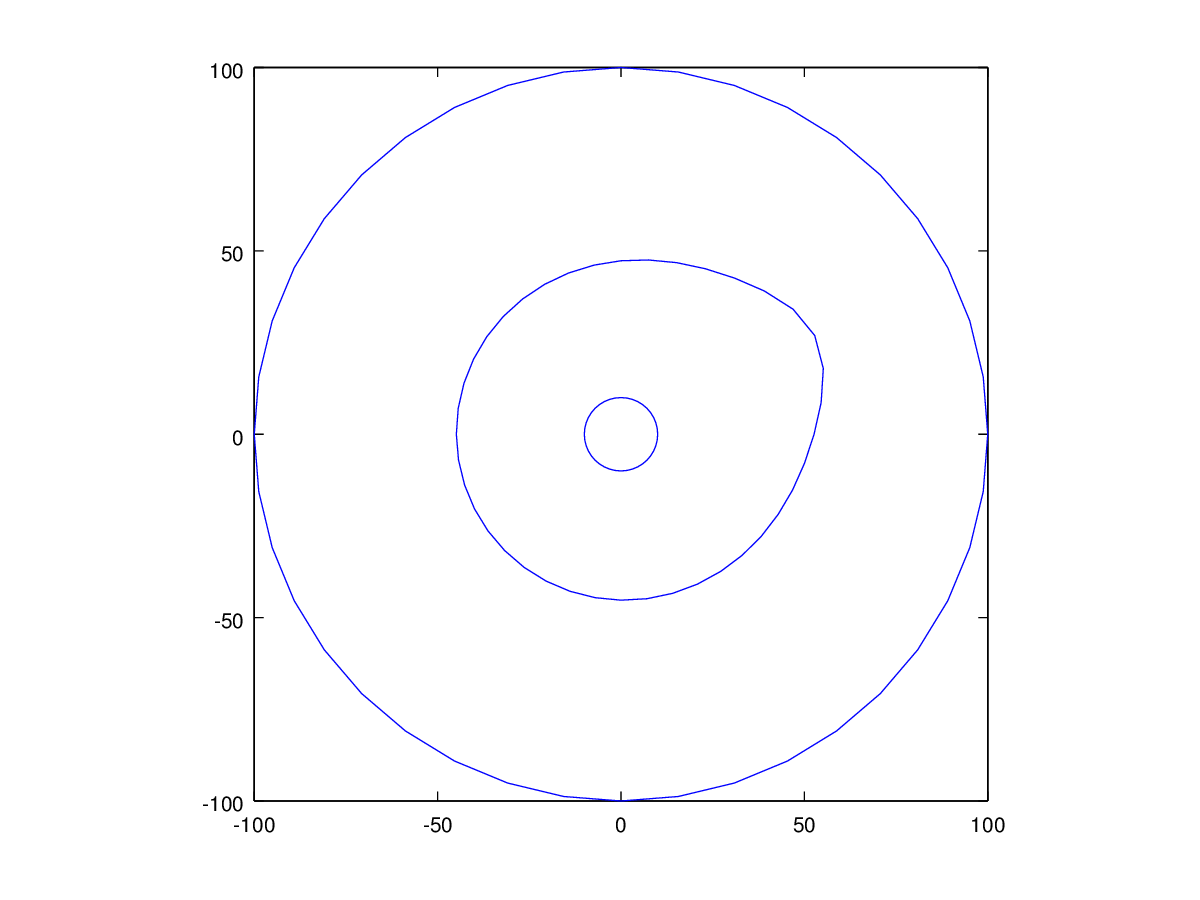
\includegraphics[width=1\textwidth]{imgs/comp_angulos/comp_angs_iso0.png}
  \caption{}
  \label{fig:comp_angs_iso0}
\end{minipage}%
\hspace{0.03\textwidth}
\begin{minipage}{0.30\textwidth}   
  \centering
    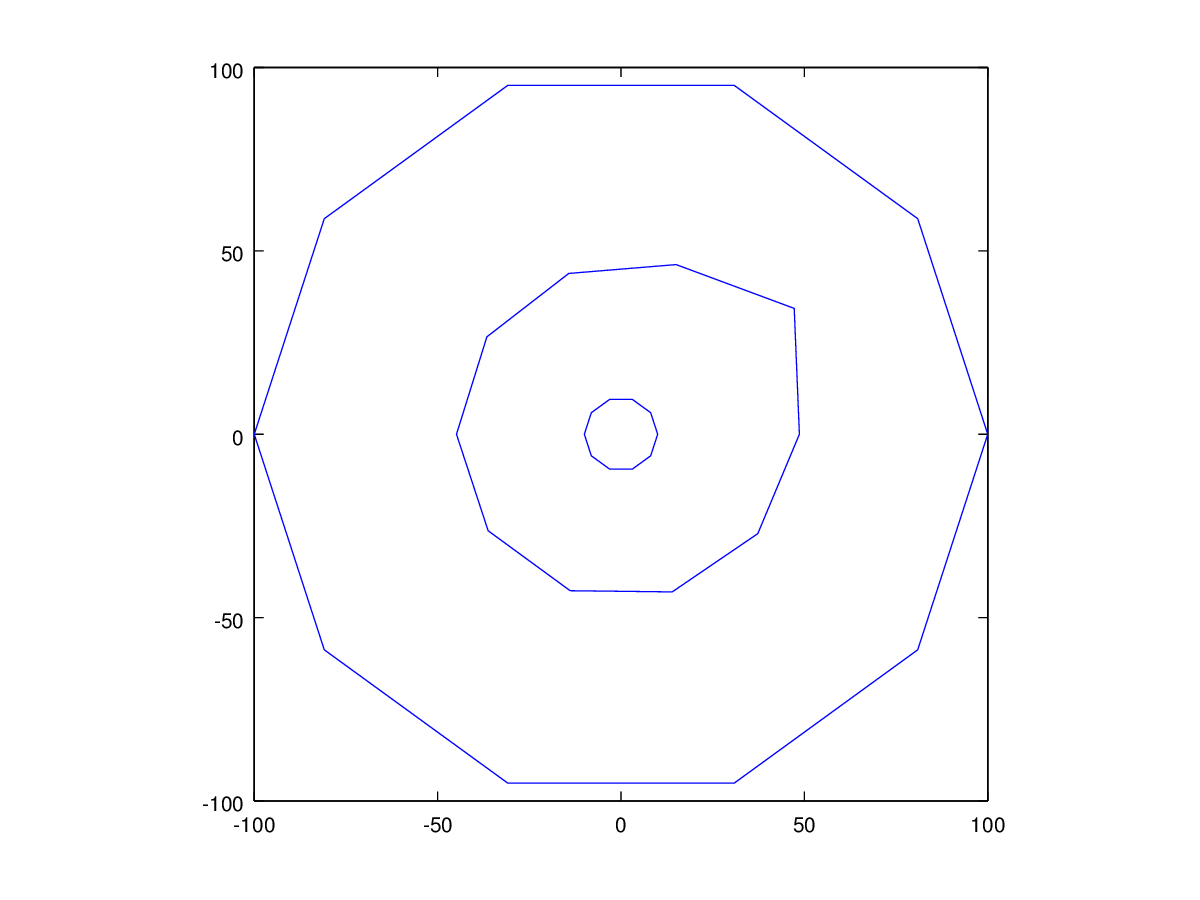
\includegraphics[width=1\textwidth]{imgs/comp_angulos/comp_angs_iso3.png} 
  \caption{}
  \label{fig:comp_angs_iso3}
\end{minipage}%
\hspace{0.03\textwidth}
\begin{minipage}{0.30\textwidth}   
  \centering
    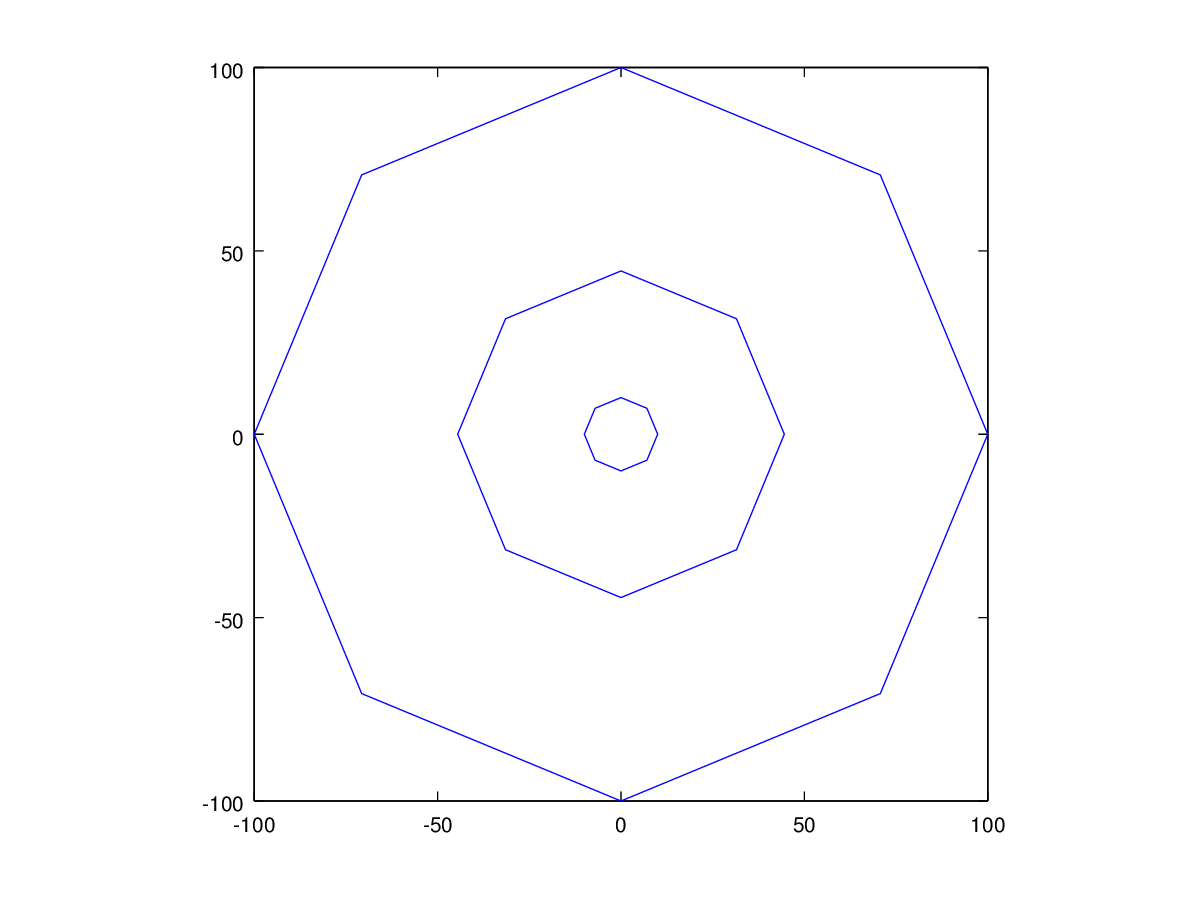
\includegraphics[width=1\textwidth]{imgs/comp_angulos/comp_angs_iso4.png} 
  \caption{}
  \label{fig:comp_angs_iso4}
\end{minipage}

\end{figure}

En la Figura \ref{fig:comp_angs_iso0}, con 30 ángulos, se puede detectar a la perfección un pico en la isoterma. Luego, en la Figura \ref{fig:comp_angs_iso3}, con 10 ángulos si bien se detecta un pico, la forma que se muestra está muy alejada de la real, esto podría causar falsas alarmas o la ausencia de las mismas.
Finalmente, en la Figura \ref{fig:comp_angs_iso4}, en la que se discretizó con 8 ángulos se puede observar como el pico desaparece fallando dramaticamente la predicción en la forma de la isoterma.

Para mas detalles de la evolución de la isoterma y las temperaturas calculadas en el sistema se recomienda recurrir al link citado mas arriba, http://bit.ly/1Uqt90x, en la animación comp_angs_iso se podrá notar con mayor detalle lo nombrado previamente, la isoterma ira marcando el pico con mayor precisión a medida que se utilicen mas ángulos, en los casos en que la cantidad de ángulos sea insuficiente el pico y las temperaturas en esa zona estaran muy distorsionadas, esto se puede observar claramente en comp_angs_temp, donde las temperaturas en la zona del pico se calculan de forma imprecisa debido a la utilización de una cantidad de ángulos muy pobre.


\subsubsection{Granularidad de los radios}
Al estudiar las posibilidades en la cantidad de radios a utilizar se puede observar como a mayor granularidad mejora la posición de la isoterma, convergiendo a la posición real. A diferencia de los ángulos, con los radios los picos serán detectados sin tomar demasiadas precauciones pero para asegurar que el tamaño de los picos, y de la isoterma en general, sean predichos de forma confiable se recomendara utilizar una cantidad de radios adecuadamente alta según la necesidad que se tenga.

Para verificar un poco esto utilizamos dos instancias de prueba. La primera forma una isoterma con forma de óvalo debido a un aumento en la temperatura externa en dos zonas opuestas. La segunda es un círculo perfecto producido por una temperatura constante a lo largo de todo el interior y exterior del horno. En ambos casos veremos como la figura va cambiando su tamaño al tender a la isoterma real.

\subsubsection{Instancia 1}

\begin{figure}[H]
\centering
\begin{minipage}{0.48\textwidth}
  \centering
    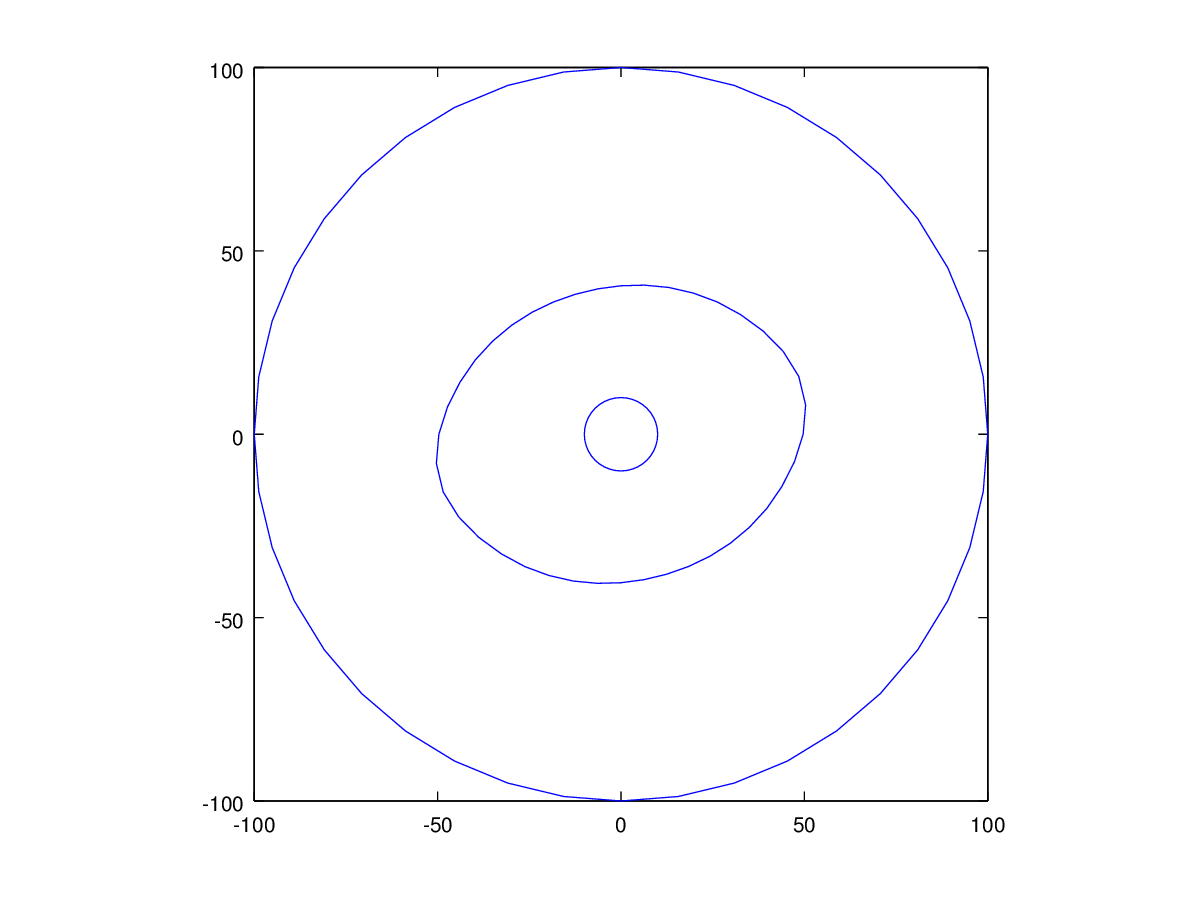
\includegraphics[width=1\textwidth]{imgs/comp_rads_bueno/comp_radss_iso5.png}
  \caption{}
  \label{fig:Radios1}
\end{minipage}%
\hspace{0.03\textwidth}
\begin{minipage}{0.48\textwidth}   
  \centering
    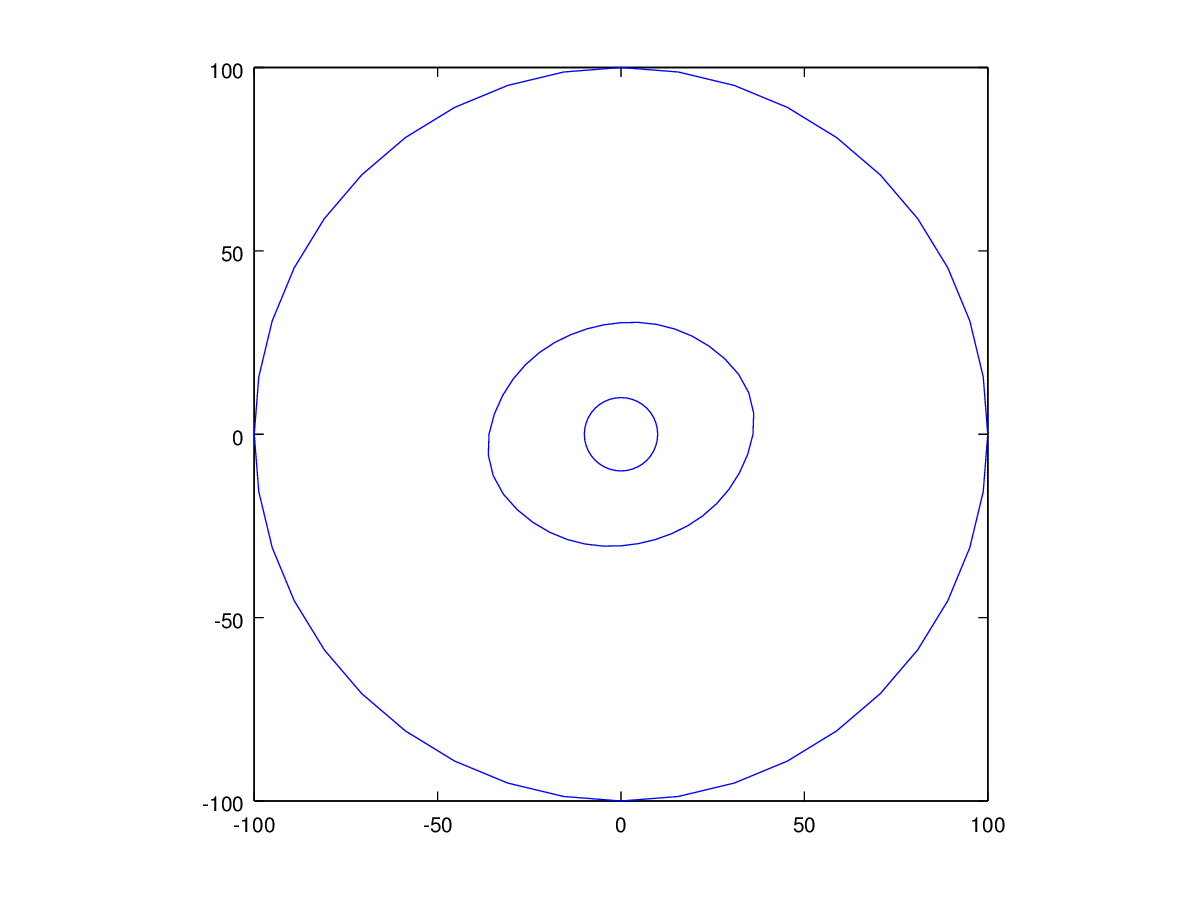
\includegraphics[width=1\textwidth]{imgs/comp_rads_bueno/comp_radss_iso0.png} 
    \caption{} 
  \label{fig:Radios2}
\end{minipage}
\end{figure}


Se puede observar como, a pesar de tener el mismo conjunto de temperaturas exteriores e interiores, y la misma discretización con respecto a los ángulos, hay una gran diferencia entre la Figura \ref{fig:Radios1}, con 30 radios, que consigue una aproximación muy buena del tamaño de la isoterma y la Figura \ref{fig:Radios2} que con sus 5 radios consigue una isoterma muy alejada de la real.

\subsubsection{Instancia 2}


\begin{figure}[H]
\centering
\begin{minipage}{0.48\textwidth}
  \centering
    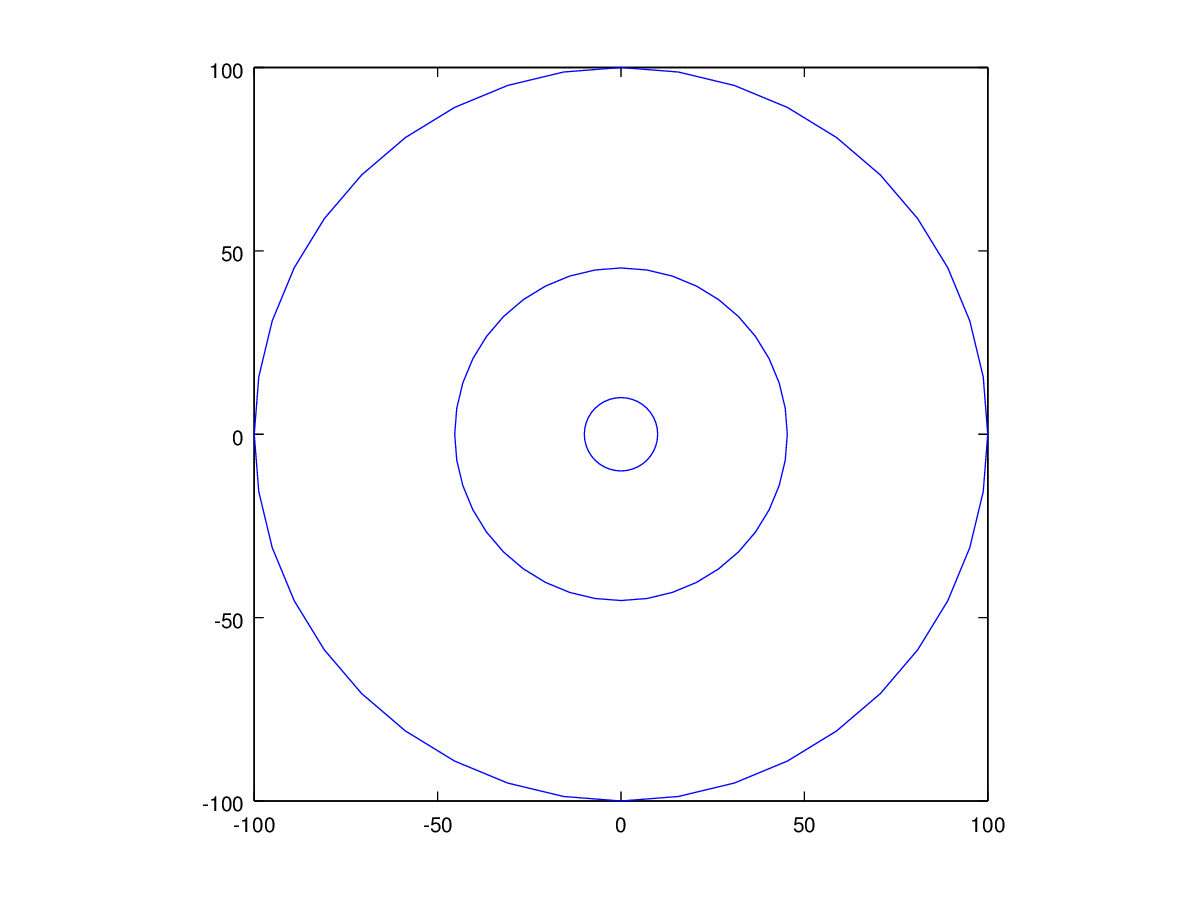
\includegraphics[width=1\textwidth]{imgs/comp_rads_malo/comp_rads_iso5.png}
	\caption{60 radios}  
  \label{fig:Radios3}
\end{minipage}%
\hspace{0.03\textwidth}
\begin{minipage}{0.48\textwidth}   
  \centering
    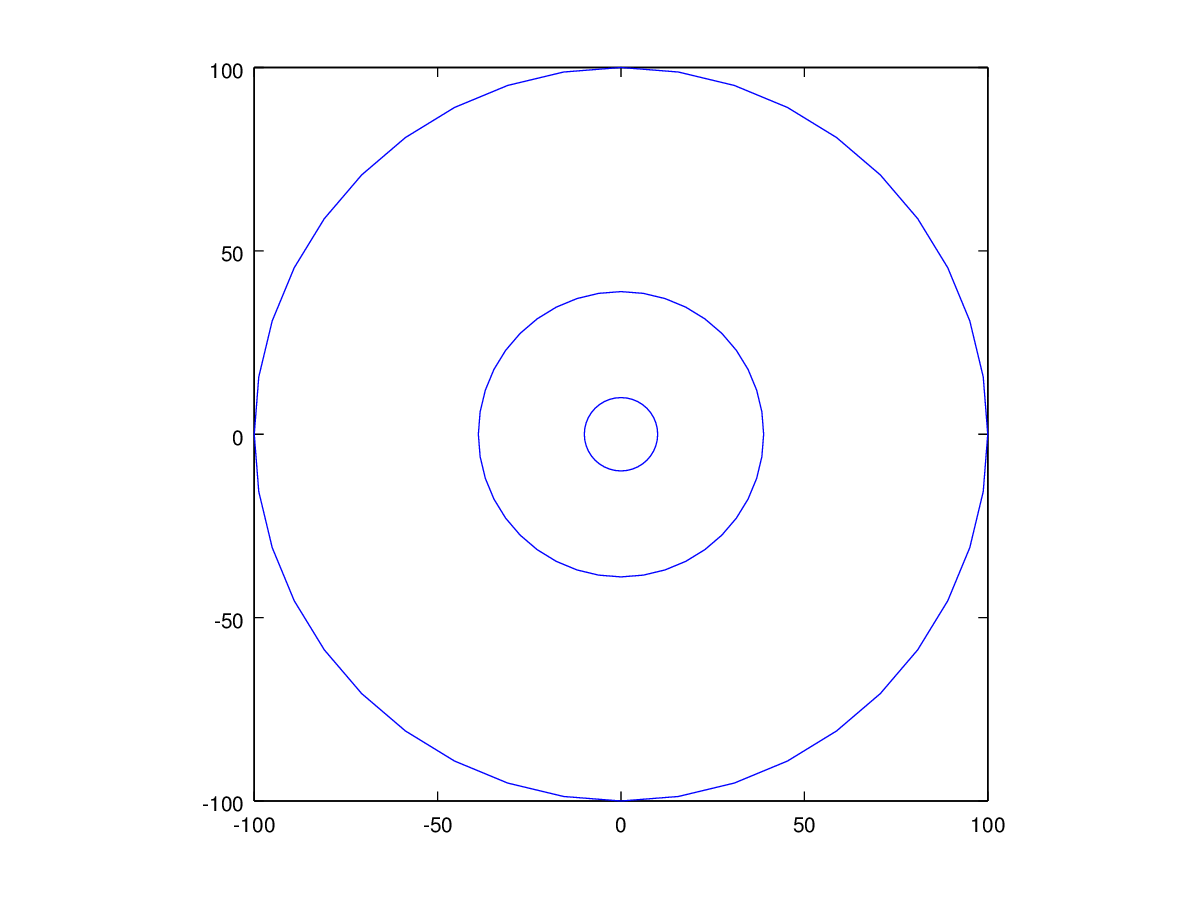
\includegraphics[width=1\textwidth]{imgs/comp_rads_malo/comp_rads_iso0.png} 
	\caption{10 radios} 
  \label{fig:Radios4}
\end{minipage}
\end{figure}

Sucede lo mismo que en en el experimento anterior, al tomar una cantidad relativamente alta de radios se logra un error muy pequeño del tamaño de la isoterma, en este caso se utilizaron 60. La diferencia entre utilizar 40, 50 y 60 radios no fue muy grande, al menos para nuestros estandares, por lo cual se podrian utilizar simplemente 40 consiguiendo un buena relacion entre tiempo de cálculo y aproximación al tamaño de la isoterma, para apreciar mejor esto pueden acceder a http://bit.ly/1Uqt90x y ver las animaciones "comp\_rads\_iso" y "comp\_rads\_iso2".


\subsection{Evaluación de los métodos}

\subsubsection{Único $b$}
Nuestro primer análisis de los métodos utilizados para la resolución del problema va a consistir en uno teórico. 

La resolución mediante el método de eliminación Gaussiana tiene dos partes, la primera es la eliminación gaussiana propiamente dicha, que tiene un costo de $O(k^3)$ flops, donde $k$ es la cantidad de filas (y columnas) de la matriz y la segunda es el algoritmo llamado \emph{backwards substitution}, que tiene un costo de $O(k^2)$ flops.

La resolución mediante el método de factorización LU tiene tres partes, la primera es obtener la factorización LU de la matriz en cuestión, que tiene un costo de $O(k^3)$, y luego aplicar \emph{forward substitution} y \emph{backward substitution}, cada uno con un costo de $O(n^2)$ flops.



Para medir los tiempos de ambas implementaciones decidimos hacer dos experimentos separados, sin embargo similares. 
En uno fijamos una cantidad de radios y movemos la cantidad de ángulos, y en el otro al revés.
Lo hicimos así para que las dimensiones de la matriz (ancho o alto, dado que son iguales porque es cuadrada) crezca linealmente, ya que si hacemos variar ángulos y radios al mismo tiempo, las dimensiones dejan de crecer linealmente.
Queremos que las dimensiones crezcan linealmente para que los resultados se entiendan mejor, dado que una escala lineal es, generalmente, más natural a la vista.


\begin{figure}[H]
\centering
\begin{minipage}{0.48\textwidth}
  \centering
    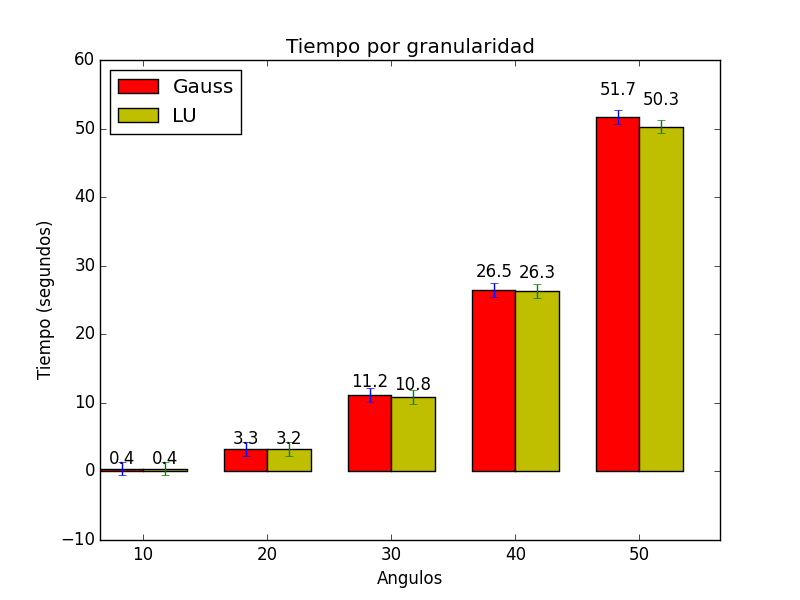
\includegraphics[width=1\textwidth]{imgs/tiempos_vanilla_angulos.png}
  \caption{\footnotesize{Tiempo tomado por nuestra implementación de eliminación gaussiana y de factorización LU para resolver el problema. La granularidad de radios está fija en 40 y la de ángulos se indica en el eje $x$. La barra principal indica el promedio, y el segmento indica la desviación standard.}}
  \label{fig:tiempo1}
\end{minipage}%
\hspace{0.03\textwidth}
\begin{minipage}{0.48\textwidth}   
  \centering
    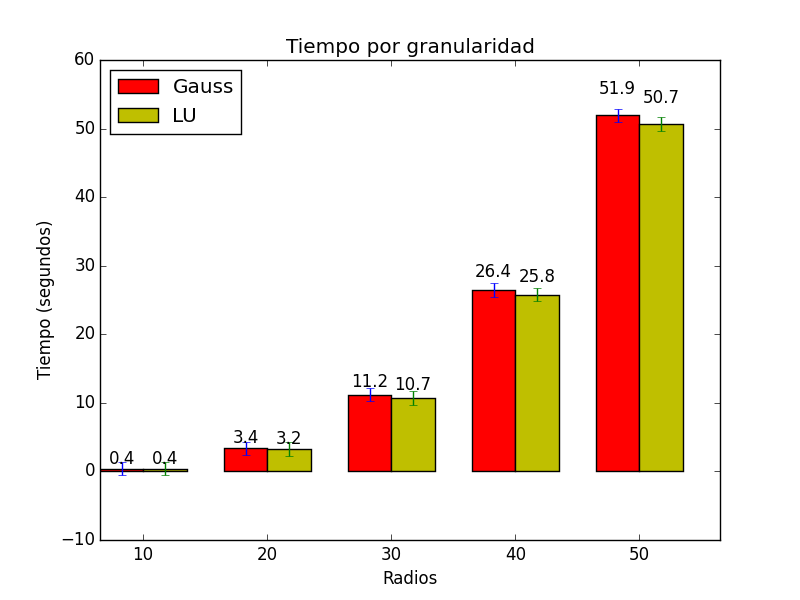
\includegraphics[width=1\textwidth]{imgs/tiempos_vanilla_radios.png} 
  \caption{\footnotesize{Tiempo tomado por nuestra implementación de eliminación gaussiana y de factorización LU para resolver el problema. La granularidad de ángulos está fija en 40 y la de radios se indica en el eje $x$. La barra principal indica el promedio, y el segmento indica la desviación standard.}}
  \label{fig:tiempo2}
\end{minipage}
\end{figure}



Como se ve en las figuras \ref{fig:tiempo1} y \ref{fig:tiempo2}, las performances entre las implementaciones son realmente similares. También puede observarse algo que nos llamó la atención, que es que el método por eliminación gaussiana tuvo consistentemente peor performance que LU, contradiciendo parcialmente el análisis \emph{a priori}. Sin embargo, la diferencia es mínima: siempre menor al 3\%.

Por esta razón no creemos que sea algo importante a tener en cuenta, y podríamos atribuirlo a optimizaciones del compilador, dado que los códigos son realmente parecidos (de hecho hicimos nuestra implementación de la factorización LU sobre nuestra implementación de eliminación gaussiana), y las partes que son diferentes le agregan complejidad a la factorización LU.

Por eso lo atribuimos a cuestiones relacionadas con la optimización en tiempo de compilación y no a errores en las mediciones, dado que los tests fueron corridos varias veces por el hecho de que estos resultados eran llamativos.


Por otro lado, vemos que dividir entre ángulos y radios no hace diferencia en la performance, dado que como esperábamos, el runtime solamente depende del tamaño de la matriz, es decir $n (m+1)$, que en ambos gráficos es igual columna a columna.


Ahora es el turno de las implementaciones que aprovechan que la matriz es banda.
La diferencia es enorme. Para comparar rápidamente, podemos usar una tabla:


\begin{figure}[H]
\centering
\begin{tabular}{|r | c  c  c  c|}
\hline
  \textbf{Implementación} & Gauss & Gauss Banda & LU & LU Banda\\ \hline
  \textbf{Tiempo (segundos)} & 26.24 & 0.98 & 25.53 & 1.04 \\
\hline
\end{tabular}

  \caption{\footnotesize{Tiempo promedio tomado por las implementaciones para resolver un sistema con $n = m+1 = 40$.}}
  \label{fig:tiempocomp}
\end{figure}

Con la Figura \ref{fig:tiempocomp} se observa como la diferencia entre las implementaciones \emph{vanilla} y las optimizadas es abismal, superando el 2600\%. Esta tabla no pretende analizar las implementaciones optimizadas, simplemente probar la diferencia de rendimiento que se obtiene, dado que poner ambas implementaciones en un mismo gráfico no nos permitiría apreciar la diferencia.

A continuación analizaremos las implementaciones optimizadas.

Como puede verse en el código, la complejidad de los algoritmos optimizados para realizar la eliminación Gaussiana (y por lo tanto la factorización LU) es $O(n^3 (m+1))$. Esto se debe a que, para cada fila (hay $n(m+1)$ filas) debemos realizar un trabajo que cuesta $O(n^2)$ flops.

Lo anterior es fácilmente justificable, porque en cada paso de la eliminación gaussiana el objetivo es poner ceros debajo de la diagonal, entonces solo debemos modificar tantas filas como cantidad de ángulos hay, dado que la matriz es banda y tiene la forma que fue explicada anteriormente.

Además de esas filas, sólo se deben modificar tantos coeficientes como ángulos, dado que sabemos que para la derecha de la fila en cuestión hay solamente ceros. Nuevamente, esto se sigue de la explicación anterior sobre la construcción de la matriz, que fue explicada anteriormente.

Debido a esto, esperamos que cueste mucho mas aumentar la granularidad con respecto a los ángulos que con respecto a los radios, como se vió reflejado en los experimentos que siguen.

\begin{figure}[H]
\centering
\begin{minipage}{0.48\textwidth}
  \centering
    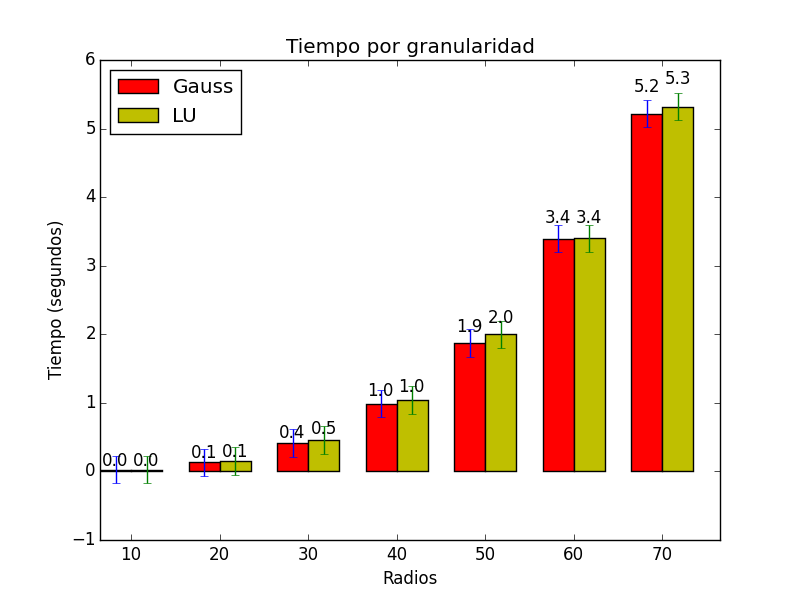
\includegraphics[width=1\textwidth]{imgs/tiempos_opt_radios.png}
  \caption{\footnotesize{Tiempo tomado por nuestra implementación optimizada de eliminación gaussiana y de factorización LU para resolver el problema. La granularidad de radios está fija en 40 y la de ángulos se indica en el eje $x$. La barra principal indica el promedio, y el segmento indica la desviación standard.}}
  \label{fig:tiempoopt1}
\end{minipage}%
\hspace{0.03\textwidth}
\begin{minipage}{0.48\textwidth}   
  \centering
    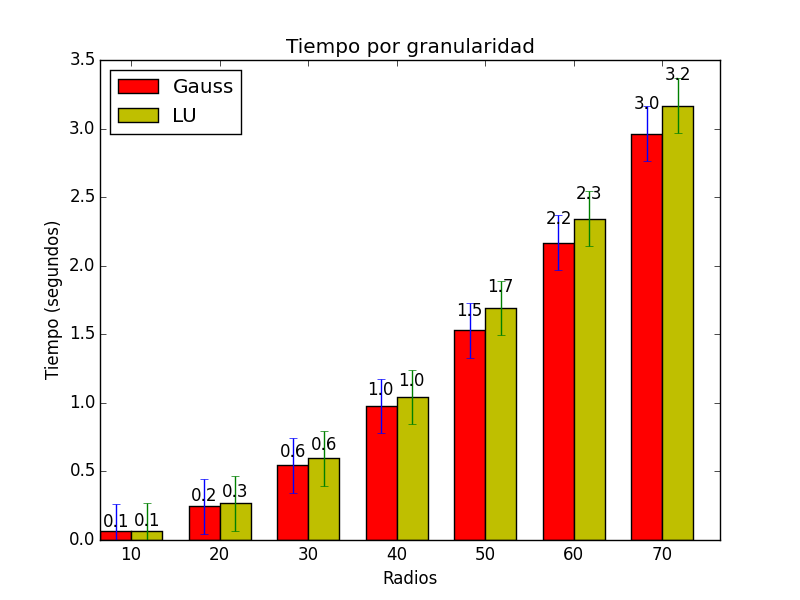
\includegraphics[width=1\textwidth]{imgs/tiempos_opt_angulos.png} 
  \caption{\footnotesize{Tiempo tomado por nuestra implementación optimizada de eliminación gaussiana y de factorización LU para resolver el problema. La granularidad de ángulos está fija en 40 y la de radios se indica en el eje $x$. La barra principal indica el promedio, y el segmento indica la desviación standard.}}
  \label{fig:tiempoopt2}
\end{minipage}
\end{figure}


Los resultados que se ven en las Figuras \ref{fig:tiempoopt1} y \ref{fig:tiempoopt2} son muy interesantes. Primero notemos que como los procesos de eliminación gaussiana y factorización LU ambos consumen menos tiempo, se nota más la ventaja que le saca gauss a LU con un solo $b$, dado que los procesos de substitución empiezan a pesar asintóticamente.


Como la complejidad de los algoritmos optimizados es $O(n^3(m+1))$, en los experimentos se refleja que es mucho más caro aumentar la granularidad con respecto a los radios que con respecto a los ángulos, como sostuvimos anteriormente.

\subsubsection{Múltiples $b$'s}

Cuando buscamos simular un escenario similar al experimento anterior, pero donde las condiciones de borde (temperaturas interiores y exteriores) cambian en distintos instantes de tiempo, la situación es muy distinta. Aquí esperaríamos ver el verdadero poder de la factorización LU.

Por esta razón, esperamos que la implementación de la factorización LU supere ampliamente a la de la eliminación Gaussiana, dado que en la Gaussiana se paga un costo cúbico cada vez que se quiere resolver el sistema, mientras que en con la factorización LU el costo cúbico se paga solo una vez.

Por esta razón se puede decir que, para muchas instancias, el costo de resolver $Ax = b$ es cúbico para la eliminación gaussiana y cuadrático amortizado para la factorización LU.

\begin{figure}[H]
\centering  
 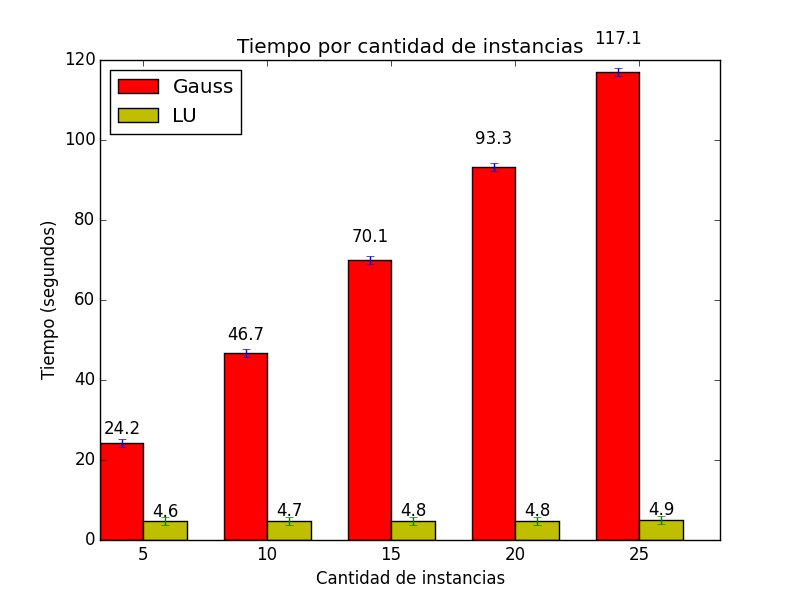
\includegraphics[width=0.6\textwidth]{imgs/tiempos_ninst.png}
 \caption{\footnotesize{Tiempo tomado por nuestra implementación de eliminación gaussiana y de factorización LU para resolver el problema para varias instancias de $n = m+1 = 30$. La barra principal indica el promedio, y el segmento indica la desviación standard.}}
\label{fig:tiemponinst}
\end{figure}


En los resultados se refleja lo que esperábamos. Como se ve en la figura \ref{fig:tiemponinst}, luego de aplicar la factorización LU, el costo que hay que pagar para resolver cada sistema es muy poco, lo cual permite una excelente performance.

Por otra parte, se observa que el tiempo que le toma a la eliminación gaussiana resolver $n$ instancias, es también es lineal en la cantidad de instancias, pero con una pendiente mucho mayor, lo cual confirma más aún nuestras expectativas derivadas de la teoría.

En cuanto a las implementaciones optimizadas, esperamos que su comportamiento sea similar a los resultados anteriores.

Con estas instancias, además de simplemente tomar tiempos, también guardamos los resultados y obtuvimos imágenes, a partir de las cuales armamos animaciones. Estas animaciones pueden verse en los links de YouTube de \ref{sec:links}.

\begin{figure}[H]
\centering  
 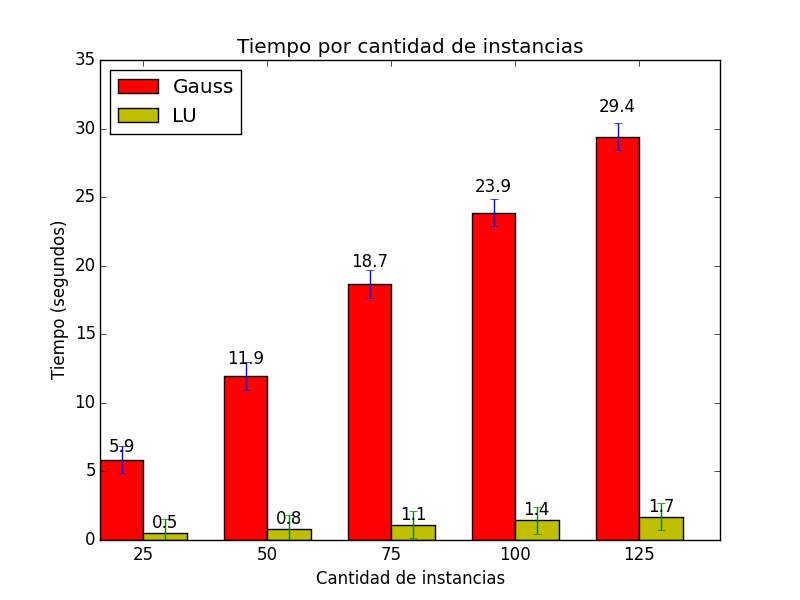
\includegraphics[width=0.6\textwidth]{imgs/tiempos_ninst_opt.png}
 \caption{\footnotesize{Tiempo tomado por la nuestra implementación optimizada de eliminación gaussiana y de factorización LU para resolver el problema para varias instancias de $n = m+1 = 40$. La barra principal indica el promedio, y el segmento indica la desviación standard.}}
\label{fig:tiemponinstopt}
\end{figure}

Como se observa en la Figura \ref{fig:tiemponinstopt}, confirmamos nuestras expectativas. Se observa, al igual que antes, que la implementación optimizada de Gauss crece linealmente con respecto a la cantidad de instancias del problema entradas, al igual que la implementación de la factorización LU, sólo que esta ultima lo hace con una pendiente mucho menor.




\newpage

\section{Conclusiones}
Para empezar, queremos decir que creemos que este trabajo práctico fue fructífero. Pudimos implementar correctamente los métodos numéricos de resolución de sistemas lineales vistos en clase, lo cual nos ayudó mucho a entenderlos e internalizarlos mucho más.

Además fue muy positiva la experiencia de utilizar estos métodos para resolver un problema de la vida real. Este TP, por otro lado, nos permitió darnos un poco de idea de cuáles son las aplicaciones más usuales de los algoritmos vistos en la materia. Otra cosa notable que se desprende de este TP es lo importante que es abarcar un problema interdisciplinariamente: en este caso necesitamos conocer la ecuación de Laplace (física), saber que una derivada se puede aproximar con un cociente incremental con diferencias finitas (matemática) y utilizar métodos numéricos para resolver sistemas de ecuaciones lineales (computación).

En la misma línea, tomar tiempos de los algoritmos y comparar sus performances nos permitió corroborar lo que ya sabíamos en la teoría de manera práctica, además de ganar intuición sobre el comportamiento de los algoritmos.

Una cosa que nos gustaría decir, es que los experimentos que llegaron al TP son sólo una pequeña proporción de todos los que realizamos. Muchos quedaron afuera porque estaban mal hechos (pocas instancias de prueba, bugs) o simplemente porque no mostraban de forma tan clara lo que queriamos expresar. De manera iterativa, llegamos a los experimentos que presentamos que, desde nuestro punto de vista, expresan perfectamente lo que queríamos que expresaran.

Pasando a las conclusiones sobre la experimentación propiamente dicha, pudimos determinar empíricamente las siguientes cuestiones:
\begin{itemize}
\item Una mayor granularidad de los ángulos que se toman en la discretización favorece a detectar picos localizados de temperaturas que podrían pasar desapercibidos de lo contrario. A su vez, una mayor granularidad de los radios permite delinear con mucha mayor precisión la isoterma. Sin embargo, como vimos, a medida que aumentamos la cantidad de radios la posición de la isoterma va convergiendo a una posición que varía cada vez menos.
\item Aumentar la granularidad de la discretización aumenta también el tiempo de cómputo requerido para resolver el sistema de ecuaciones. Para el caso en que sólo se pasa una instancia, los métodos de eliminación gaussiana y de factorización LU muestran una performance casi idéntica, mientras que en el caso en que se toman múltiples instancias vemos como la factorización LU supera ampliamente a la eliminación gaussiana, confirmando lo que se esperaba desde la teoría (la complejidad de eliminación gaussiana es cúbica para resolver cada instancia, mientras que LU tiene un costo amortizado cuadrático). Por otro lado, las versiones optimizadas que aprovechan el hecho de que la matriz sea banda demostraron ser por mucho superiores a sus contrapartes tradicionales.
\item Por los dos puntos anteriores, es posible encontrar una granularidad \emph{óptima} (en algún sentido) tal que la isoterma obtenida sea lo suficientemente precisa sin pagar un costo en tiempo de cómputo excesivo, pues dijimos que al aumentar los radios la posición de la misma convergía, llegando un punto en el que un aumento de la granularidad produce una difertencia mínima en el resultado.
 \end{itemize}

Para finalizar, nos gustaría plantear trabajo a futuro, y atar algunos cabos sueltos. Nuestra implementación \emph{optimizada} de los algoritmos de eliminación gaussiana y factorización LU que aprovechaban el hecho de que la matriz es banda, solamente tenía una ganancia de performance con respecto al tiempo, dado que seguimos almacenando la matriz en un vector de vectores.

Por esa razón, es interesante plantearse el problema de como llevar a cabo esta optimización de la complejidad espacial de nuestros métodos. Algunas ideas en lo que respecta a la solución de este problema pueden hallarse en \cite[Cap. 4.3]{golub}. 





\section{Apéndices}
\subsection{Demo}
Primero observemos que A es una matriz diagonal dominante no estricta. Para eso tenemos que ver que para cada fila el valor absoluto de la diagonal es mayor o igual que la norma-1 del resto de los elementos de esa fila. En nuestro caso puntual, esto significa ver que 
$|b_k| \geq |a_k| + 2|c_k| + |d_k|$. 

Primero calculemos el lado derecho de la desigualdad:
\begin{equation*}
\left\vert \dfrac{r_k - \Delta r}{r_k (\Delta r)^2}\right\vert +
2 \times \left\vert \dfrac{1}{r_k^2(\Delta \theta)^2} \right\vert+
\left\vert \dfrac{1}{(\Delta r)^2} \right\vert = 
\dfrac{\left\vert r_k - \Delta r \right\vert}{r_k (\Delta r)^2} +
2 \times \dfrac{1}{r_k^2(\Delta \theta)^2} +
\dfrac{1}{(\Delta r)^2}
\end{equation*}

Asumamos primero que $\left\vert r_k - \Delta r \right\vert \geq 0$. En ese caso la ecuación anterior es igual a
 
\begin{center}
$\dfrac{2 r_k^2 (\Delta \theta)^2 - (\Delta r) r_k (\Delta \theta)^2 + 2 (\Delta r)^2}{r_k^2 (\Delta r)^2 (\Delta \theta)^2}$
\end{center}

Entonces, queremos ver que $|b_k|$ es mayor o igual que eso, es decir

\begin{equation*}
\dfrac{\left\vert -2 r_k^2 (\Delta \theta)^2 + (\Delta r) r_k (\Delta \theta)^2 - 2 (\Delta r)^2 \right\vert } 
{\left\vert r_k^2 (\Delta r)^2 (\Delta \theta)^2 \right\vert } \geq
\dfrac{2 r_k^2 (\Delta \theta)^2 - (\Delta r) r_k (\Delta \theta)^2 + 2 (\Delta r)^2}{r_k^2 (\Delta r)^2 (\Delta \theta)^2}
\end{equation*}

Que es equivalente a

\begin{equation*}
\left\vert -2 r_k^2 (\Delta \theta)^2 + (\Delta r) r_k (\Delta \theta)^2 - 2 (\Delta r)^2 \right\vert \geq
2 r_k^2 (\Delta \theta)^2 - (\Delta r) r_k (\Delta \theta)^2 + 2 (\Delta r)^2
\end{equation*}

Supongamos que lo que está dentro del módulo es positivo, entonces tenemos

\begin{center}
$-2 r_k^2 (\Delta \theta)^2 + (\Delta r) r_k (\Delta \theta)^2 - 2 (\Delta r)^2 \geq
2 r_k^2 (\Delta \theta)^2 - (\Delta r) r_k (\Delta \theta)^2 + 2 (\Delta r)^2$ \\
$\Updownarrow$\\
$2\times (-2 r_k^2 (\Delta \theta)^2 + (\Delta r) r_k (\Delta \theta)^2 - 2 (\Delta r)^2) \geq 0$\\
$\Updownarrow$\\
$-2 r_k^2 (\Delta \theta)^2 + (\Delta r) r_k (\Delta \theta)^2 - 2 (\Delta r)^2 \geq 0$
\end{center}

Pero esta última desigualdad vale pues habíamos supuesto que efectivamente eso era positivo.

Ahora veamos que pasa si lo de adentro del módulo es negativo. Tenemos que 

\begin{center}
$-2 r_k^2 (\Delta \theta)^2 + (\Delta r) r_k (\Delta \theta)^2 - 2 (\Delta r)^2 \leq
-2 r_k^2 (\Delta \theta)^2 + (\Delta r) r_k (\Delta \theta)^2 - 2 (\Delta r)^2$ \\
$\Updownarrow$\\
$0 \leq 0$\\
\end{center}

Que vale trivialmente. Luego probamos que la matriz del sistema es diagonal dominante no estricta, si $~{\left\vert r_k - \Delta r \right\vert \geq 0}$. Notar además que por la última cuenta no es cierto que sea diagonal dominante estricta.
\end{document}
